\documentclass[12pt,notitlepage]{article}
\author{Leo Przybylski \\
\texttt{przybyls@u.arizona.edu}}
\usepackage{graphicx}
\usepackage{listings}
\usepackage{color}
\usepackage{hyperref}
\usepackage{hyperlatex}
\setcounter{htmldepth}{0}

\definecolor{DarkBlue}{rgb}{0,0,0.55}
\definecolor{DarkGreen}{rgb}{0,0.4,0}
\definecolor{Purple}{rgb}{0.5,0,0.5}

\begin{ifhtml}
\newcommand{\sf}[1]{\xml{span style="font-family: sans-serif;"}#1\xml{/span}}
\newcommand{\rm}[1]{\xml{span style="font-family: serif;"}#1\xml{/span}}
\newcommand{\bf}[1]{\xml{span style="font-weight: bold;"}#1\xml{/span}}
\newcommand{\href}[2]{\xml{a href="#1"}#2\xml{/a}}
\newcommand{\HlxStyleSheet}{
  \begin{rawxml}
    <!-- metadata -->
    <meta name="generator" content="S5" />
    <meta name="version" content="S5 1.1" />
    <meta name="presdate" content="\end{rawxml}\HlxDate\begin{rawxml}"/>
    <meta name="author" content="\end{rawxml}\HlxAuthor\begin{rawxml}"/>
    <meta name="company" content="Leosandbox " />
    <!-- configuration parameters -->
    <meta name="defaultView" content="slideshow" />
    <meta name="controlVis" content="hidden" />
    <!-- style sheet links -->
    <link rel="stylesheet" href="ui/kuali/slides.css" type="text/css" media="projection" id="slideProj" />
    <link rel="stylesheet" href="ui/kuali/outline.css" type="text/css" media="screen" id="outlineStyle" />
    <link rel="stylesheet" href="ui/kuali/print.css" type="text/css" media="print" id="slidePrint" />
    <link rel="stylesheet" href="ui/kuali/opera.css" type="text/css" media="projection" id="operaFix" />
    <script src="ui/kuali/slides.js" type="text/javascript"></script>
  \end{rawxml}
}

\newcommand{\maketitle}{
    \xml{div class="slide"}
    \EmptyP{\HlxTitleP}{\HlxBlk\xml{h1}\HlxTitle\xml{/h1}
    \EmptyP{\HlxAuthorP}{\xml{h2}\HlxAuthor\xml{/h2}}{}
    \EmptyP{\HlxDate}{\xml{h3}\HlxDate\xml{/h3}}{}
    \xml{/div}
    }{}}

\end{ifhtml}

\newenvironment{s5presentation}{\endpar%
  \HlxBlk\begin{rawxml}
  <div class="header">
    <div class="header_l">
      <div class="header_r">
      &nbsp;
      </div>
    </div>
  </div>
  <div class="content">
    <div class="content_l">
      <div class="content_r">
        <img src="ui/kuali/blank.gif" id="filler" border="0"/>
<div class="layout">
  <div id="controls"><!-- DO NOT EDIT --></div>
  <div id="currentSlide"><!-- DO NOT EDIT --></div>
  <div id="header">
    <img style="position: relative; top:30px; left: 18px;" src="ui/kuali/logo.png" />
  </div>
  <div id="footer">
    <div class="footer_l">
      <div class="footer_r">
        <h1/>
        <h2>\end{rawxml}\HlxTitle\begin{rawxml}</h2>
      </div>
    </div>
  </div>
</div>
    </div>
  </div>
 </div>
<div class="presentation">
    \end{rawxml}}{\HlxBlk\xml{/div}}
\newenvironment{s5slide}{\xml{div class="slide"}}{\xml{/div}}
\newcommand{\fulltitle}[1]{\title{#1}\htmlonly{\htmltitle{#1}}}

\fulltitle{Inheritance vs. Encapsulation}

\newcommand{\Encapsulation}{\sf{\href{http://en.wikipedia.org/wiki/Information_hiding}{Encapsulation}}\rm{}}
\newcommand{\Abstraction}{\sf{\href{http://en.wikipedia.org/wiki/Abstraction}{Abstraction}}\rm{}}
\newcommand{\Inheritance}{\sf{\href{http://en.wikipedia.org/wiki/Inheritance_(computer_science)}{Inheritance}}\rm{}}
\newcommand{\ObjectModel}{\sf{\href{http://en.wikipedia.org/wiki/Object_model}{Object Model}}\rm{}}
\newcommand{\Modularity}{\sf{\href{http://en.wikipedia.org/wiki/Modularity_(programming)}{Modularity}}\rm{}}
\newcommand{\Polymorphism}{\sf{\href{http://en.wikipedia.org/wiki/Type_polymorphism}{Polymorphism}}\rm{}}
\newcommand{\MultiInheritance}{\sf{\href{http://en.wikipedia.org/wiki/Multiple_inheritance}{Multiple-Inheritance}}\rm{}}
\newcommand{\Kuali}{\emph{\href{http://www.kuali.org}{Kuali}}\rm{}}
\newcommand{\KualiFinancialSystem}{\emph{\href{http://www.kuali.org}{Kuali Financial System}}\rm{}}
\newcommand{\KFS}{\emph{\href{http://www.kuali.org}{KFS}}}

\begin{document}
  \texonly{
    \lstset{language=Java,
      basicstyle=\small,
      keywordstyle=\color{Purple}\bfseries,
      commentstyle=\color{DarkGreen},
      identifierstyle=\color{DarkBlue},
      rangeprefix=\/\/\ ,
      rangesuffix=,
      breaklines=true,
      breakatwhitespace=true,
      includerangemarker=false}
  }
  \W \begin{s5presentation}
  \maketitle
  \texonly{\tableofcontents}
  \W \begin{s5slide}
    \begin{abstract}
      \begin{ifhtml}
      \begin{itemize}
        \item Some may already know a lot of this (it's for context.)
        \item Try to quickly move passed boring material, but without ignoring context.
        \item Do not be distracted by the fancy drawings.
        \item Leo's $10^{th}$ anniversary is March 27, 2007
        \item \href{http://en.wikipedia.org/wiki/Education_and_Sharing_day}{March 27 is...}
      \end{itemize}
      \end{ifhtml}
      \begin{tex}
      Some may already know a lot of this material, and that's fine. It's mostly there for context.
      If you feel the need to move passed the boring stuff, be careful not to ignore the context. Also,
      try not to be too distracted by the pretty drawings.
      
      March 27, 2007 is Leo's $10^{\mbox{th}}$ anniversary. \href{http://en.wikipedia.org/wiki/Education_and_Sharing_day}{March 27 is also...}
      \end{tex}
    \end{abstract}
    \W \end{s5slide}
  
  \W \begin{s5slide}
    \section{\hfill Introduction}
    \T \hrulefill
    \T \\

    There are some instances in \KualiFinancialSystem\ where \Inheritance\ is possibly misused where \Encapsulation\ may have not
    only been a better fit, but may have also lessened or even eliminated the need for refactoring. This document explains how 
    \Encapsulation\ can mitigate the need for future refactorings. \Inheritance\ as it is now in Java limits modularity and orthogonal design.
    \W \end{s5slide}

    \begin{ifhtml}
      \begin{s5slide}
        \section{\hfill Introduction}
      \begin{itemize}
      \item The \ObjectModel
        \begin{itemize}
          \item Origins of \Inheritance\ and \Encapsulation
          \item \Inheritance\ and \Encapsulation\ Defined
        \end{itemize}
      \item What is the Problem?
      \item Comparing \Inheritance\ and \Encapsulation\
        \begin{itemize}
          \item How do They Differ?
          \item Labor Distribution Scenario
          \item General Ledger Scenario
          \item Struts/Spring Scenario (aka. Encapsulating Actions or Does Spring + Struts = String?)
          \item Banana Splits
          \item Solving Parallel Hierarchies
        \end{itemize}
      \item What about \texttt{abstract} Classes?
      \end{itemize}
      \end{s5slide}
    \end{ifhtml}

    \W \begin{s5slide}
      \W \section{The Object Model}
      \begin{quote}
        For all things object-oriented, the conceptual framework is the \ObjectModel. --Grady Booch ~\cite{gbone}
      \end{quote}
      
    The object model Grady Booch refers to is made up of \Abstraction, \Encapsulation, \Modularity\, and \emph{Hierarchy}.
    People have different ideas about what \Inheritance\ is. 
    \W \end{s5slide}
  
  \W \begin{s5slide}
    \texorhtml{\subsection{\Inheritance\ and \Encapsulation\ Defined}}
    {\section{Inheritance and\\ Encapsulation Defined}}
    It is important to establish such definitions to have a clear understanding
    of what is being discussed. For this document, I use the following definitions:
    \begin{ifhtml}
    \begin{itemize}
    \item What Does "\Inheritance" Mean for this Presentation?
    \item What Does "\Encapsulation" Mean for this Presentation?
    \end{itemize}
    \end{ifhtml}
  \W \end{s5slide}
  
  \begin{description}
    \W \begin{s5slide}
      \W \section{Inheritance is\ldots}
    \item[\Inheritance] is if and only if the \texttt{extends} directive is used with the \texttt{class} or \texttt{interface} clause. 
      It is important to understand that Java does not support \MultiInheritance. Java can achieve \Polymorphism by a \texttt{class} 
      implementing an \texttt{interface}.
      
      See the following example:
      \W \end{s5slide}
    
    \T \newpage
      \W \begin{s5slide}
        \section{An Inheritance Example}
        \begin{figure}[!h]
          \caption{An Inheritance Example in UML}
          \begin{ifhtml}
            \begin{verbatim}
public abstract class AbstractGLLookupableImpl 
    extends KualiLookupableImpl {
    ...
    ...
}        
        \end{verbatim}
        
        \center{\htmlimg{Diagrams/InheritanceExample_class.png}{Inheritance Example}}
          \end{ifhtml}
          \T 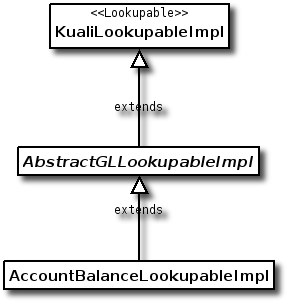
\includegraphics[bb=90 20 350 350]{Diagrams/InheritanceExample_class.png}
        \end{figure}
      \W \end{s5slide}
      \T \newpage
    \begin{tex}
      \lstinputlisting[linerange=ClassSignatureStart-ClassSignatureEnd,
                        caption={\Inheritance\ Definition Example}]{src/inheritance/AbstractGLLookupableImpl.java}
      \begin{lstlisting}
    ...
    ...
}
      \end{lstlisting}

      \begin{quote}
        Semantically, \Inheritance\ denotes an ``is-a'' relationship. \ldots 
        \Inheritance\ thus implies a genralization/specialization hierarchy, 
        wherein a subclass specializes the more general structure or behavior of its superclasses. --Grady Booch ~\cite{gbtwo}
      \end{quote}
      Based on the above quote from Grady Booch, we can assume that \Inheritance\ forms a kind of hierarchy which is an element in the 
      \ObjectModel.

      Java does not support \MultiInheritance. The only hierarchy choice is for single-inheritance through the \texttt{extends} clause as
      described above. Simply put:
      \begin{description}
      \item[Single-\Inheritance] is when one class inherits from a single superclass. The visual representation of such a hierarchy always looks
        like a tree.
      \end{description}
      \end{tex}

      \W \begin{s5slide}
        \W \section{Encapsulation is...}
        \item[\Encapsulation] is a technique of enclosing class functionality through object instances within another class. Many 
          design patterns employ \Encapsulation. Among these patterns are Delegate/Aggregate, Composite, Decorator, and Adapter (some may know these
          patterns by other names.) \Encapsulation\ can be by implementation (as in implementing and abstraction,) or aggregation.  Grady Booch 
          calls aggregation a ``part of'' relationship. See the following example:
          \W \end{s5slide}
      
      \begin{ifhtml}
        \begin{s5slide}
          \section{An Encapsulation Example}
          \href{http://en.wikipedia.org/wiki/Dependency_Injection}{Dependency Injection} is a very widely-used example of \Encapsulation\
          throughout \KFS. Basically, \href{http://en.wikipedia.org/wiki/Dependency_Injection}{Dependency Injection} achieves \emph{Loose Coupling}
          or \Modularity\ by  encapsulating functionality from other classes through delegating the implementations.
        \end{s5slide}
      \end{ifhtml}
  \end{description}

  \begin{tex}
  In simple terms, inheritance and encapsulation are both intended for implementation. Inheritance can be called an ``is a'' relationship, and
  encapsulation can be called a ``part of'' relationship type. Inheritance and encapsulation are both complementary to abstraction.
  \end{tex}

  \W \begin{s5slide}
    \W \section{What is the Problem?}
    \T \subsection{What is the Problem?}
    The problem is that Java supports \Polymorphism, but not \MultiInheritance. 
    Single-\Inheritance\ creates a single hierarchy that resembles a tree where there 
    is only one class at the very top (eg., for \sf{Java}, the \texttt{Object} class is the top-most class in the hierarchy.)
    Resulting from the lack of \MultiInheritance, Java developers have designed object-oriented 
    patterns to sidestep single-\Polymorphism\ using \Encapsulation\ rather than \Inheritance.
    \W \end{s5slide}

  \begin{tex}
    \begin{itemize}
    \item Java only has single-inheritance
    \item In order to achieve \Polymorphism\ and somewhat \MultiInheritance, Java uses \texttt{interfaces}.
    \item Interfaces are abstractions
    \item Java has a confusing \texttt{abstract} class
    \end{itemize}
    
    \subsection{What to Look Out For}
    These are concerns that will be addressed later in the document.
    \begin{itemize}
    \item When to use \Inheritance?
    \item When to use \Encapsulation?
    \item What are examples of \Encapsulation\ in Kuali
    \item What are patterns of bad uses of \Inheritance?
    \item When is the \texttt{abstract} class necessary?
    \end{itemize}

  \end{tex}

  \section{\hfill Comparing \Inheritance\ and \Encapsulation: How do They Differ?}
  \T \hrulefill
  \T \\
  \texonly{This has already been discussed in gross detail. Now we are going to show more examples
  of the differences and explain them. In this section, we will go through different scenarios
  to explore the differences. Here are some basic bullet points.}
    \W \begin{s5slide}
      \W \section{How Do They Differ?}
      \begin{itemize}
      \item They are different kinds of relationships
        \begin{itemize}
          \item \Inheritance\ is an "is a" relationship type
          \item \Encapsulation\ is a "part of" relationship type
          \end{itemize}
        \item \Modularity\ and Coupling
          \begin{itemize}
          \item \Inheritance\ leads to tight coupling
          \item \Encapsulation\ leads to loose coupling
          \end{itemize}
        \item In the \ObjectModel
          \begin{itemize}
          \item \Inheritance\ builds hierarchy
          \item \Encapsulation\ is the implementation of an \Abstraction\ which are
            combined for \Modularity
          \end{itemize}
        \item \Polymorphism
      \end{itemize}
    \W \end{s5slide}

    \begin{tex}
      \subsection{Isn't \Inheritance\ a Good Thing?}
      Not always. As it has been mentioned before, \Inheritance\ is used to build up the Hierarchy.
      Basically, that means it adds structure to whatever your Model is. Since it is an ``is a'' relationship,
      the structure is intended to be pretty concrete.
      
      \subsection{Why is \Encapsulation\ Better than \Inheritance?}
      \Encapsulation\ is the implementation to your \Abstraction. Some may be thinking now, 
      ``Isn't \Inheritance\ also implementation?'' It is, but not for an \Abstraction. Since \Inheritance\ 
      is building concrete structure to your Model, it is constricting with \Abstraction. If you 
      consider that Implementation and \Abstraction\ are what make your application Modular, then
      \Inheritance\ is actually taking away the \Modularity.
      
      Simply put, ``If you want your application to be more Modular, use \Encapsulation\ and \Abstraction\ 
      more liberally.'' If you want to rely on a more strict Model (say for strict typing) use \Inheritance.
      
      In most cases, you will want to use \Encapsulation\ and \Abstraction\ because in most cases
      you are trying to develop Orthogonal and Modular code.
      
      \subsection{Scenarios}
    \end{tex}
    
      \W \begin{s5slide}
        \T \subsubsection{Labor Distribution Scenario}
        \W \section{Labor Distribution Scenario}
        In Labor we were faced with the problem of reusing the General Ledger without refactoring it ... a lot, and 
        without introducing weird design quirks into Labor Distribution. In simple terms, ``Reuse GL, but don't 
        mess it up, don't reuse anything unnecessary, and don't be lame.''

        This is where our \Encapsulation\ is \href{http://en.wikipedia.org/wiki/Dependency_Injection}{Dependency Injection}.
        With \href{http://en.wikipedia.org/wiki/Dependency_Injection}{Dependency Injection}, we were able to reuse 
        all the interfaces within Labor and by \Encapsulation\ of functionality from the General Ledger, we were able to 
        pick and choose what was important for us to reuse and what we didn't care about. True \Modularity.
        \W \end{s5slide}

      \W \begin{s5slide}
        \W \section{How we Did it}
        \begin{figure}[!h]
            \W \center{\htmlimg{Diagrams/ScrubberValidator_validateTransactions_class.png}{Encapsulation Solution}}
          \T 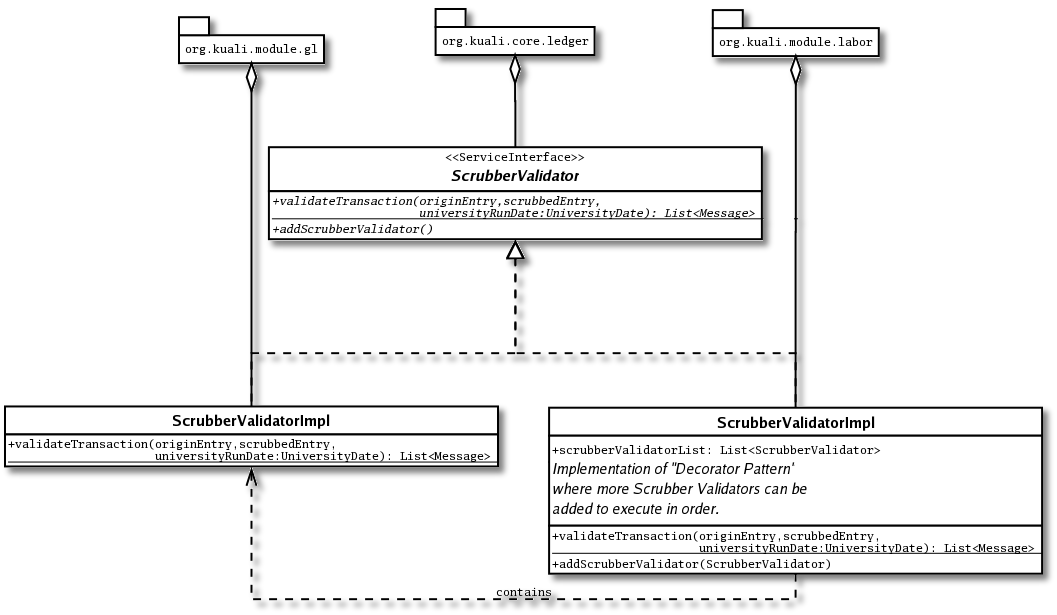
\includegraphics[bb=75 100 550 400]{Diagrams/ScrubberValidator_validateTransactions_class.png}
        \end{figure}
      \W \end{s5slide}


    \W \begin{s5slide}
      \W \section{General Ledger Scenario}
      \begin{figure}[!h]
        \caption{The Old General Ledger Account Balance Lookup Hierarchy}
        \W \center{\htmlimg{Diagrams/GlLookupableImpl_class.png}{General Ledger Account Balance Lookupable}}
        \T 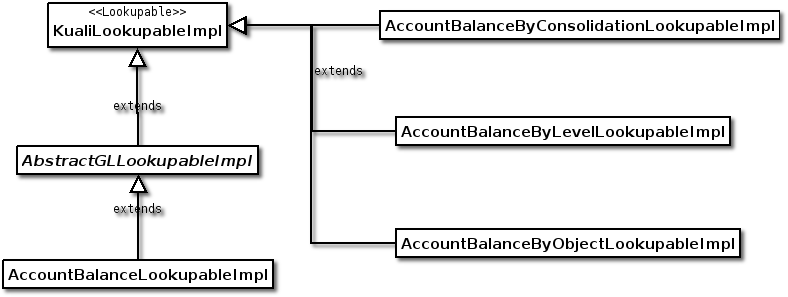
\includegraphics[bb=100 100 500 300]{Diagrams/GlLookupableImpl_class.png}
      \end{figure}
    \W \end{s5slide}

  \begin{ifhtml}
    \begin{s5slide}
      \W \section{General Ledger Scenario}
      \W \subsubsection{Further Explanation in the Handout}
    \end{s5slide}
  \end{ifhtml}

  \begin{tex}
    \subsubsection{General Ledger \Inheritance\ Scenario}

      \lstinputlisting[linerange=ClassSignatureStart-ClassSignatureEnd]{src/inheritance/AccountBalanceByConsolidationLookupableImpl.java}
      \begin{lstlisting}
    ...
    ...
}
      \end{lstlisting}
      \lstinputlisting[linerange=ClassSignatureStart-ClassSignatureEnd]{src/inheritance/AccountBalanceByLevelLookupableImpl.java}
      \begin{lstlisting}
    ...
    ...
}
      \end{lstlisting}
      \lstinputlisting[linerange=ClassSignatureStart-ClassSignatureEnd]{src/inheritance/AccountBalanceByObjectLookupableImpl.java}
      \begin{lstlisting}
    ...
    ...
}
      \end{lstlisting}
      \lstinputlisting[linerange=ClassSignatureStart-ClassSignatureEnd]{src/inheritance/AccountBalanceLookupableImpl.java}
      \begin{lstlisting}
    ...
    ...
}
      \end{lstlisting}
      
      Between \sf AccountBalanceByConsolidationLookupableImpl, AccountBalanceByLevelLookupableImpl, \rm and \sf 
      AccountBalanceByObjectLookupableImpl, \rm there isn't any \Modularity.  \Inheritance\ killed the \Modularity\ 
      with \sf KualiLookupableImpl \rm and \sf AbstractGLLookupableImpl.

      \subsubsection{General Ledger \Encapsulation\ Scenario}
      How does \Encapsulation\ fix this?
  \end{tex}

      \W \begin{s5slide}
        \W \section{How does Encapsulation Fix This?}
        \begin{figure}[!h]
          \begin{ifhtml}
            \center{\htmlimg{Diagrams/GlLookupableImplEncapsulated_class.png}{Encapsulation Solution}}
          \end{ifhtml}
          \T 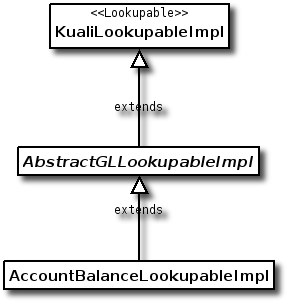
\includegraphics[bb=75 100 550 400]{Diagrams/InheritanceExample_class.png}
        \end{figure}
      \W \end{s5slide}
      
      \begin{tex}
      \begin{enumerate}
        \item Eliminate the \texttt{abstract} class
          \sf AbstractGLLookupableImpl \rm becomes \sf GlLookupableImpl\rm.
          \begin{enumerate}
            \item Rename the class and remove \texttt{abstract}
              \lstinputlisting[linerange=ClassSignatureStart-ClassSignatureEnd]{src/encapsulation/GlLookupableImpl.java}
              \begin{lstlisting}
    ...
    ...
}
              \end{lstlisting}
            \item Create new interfaces for any/all \texttt{abstract} methods
              \lstinputlisting[linerange=ClassSignatureStart-ClassSignatureEnd]{src/encapsulation/EntryCollectionUpdatable.java}
              \lstinputlisting[linerange=ClassSignatureStart-ClassSignatureEnd]{src/encapsulation/SearchableBy.java}
            \item Make \sf AccountLookupableImpl\rm implement interfaces for \texttt{abstract} method declarations
              \lstinputlisting[linerange=ClassSignatureStart-ClassSignatureEnd]{src/encapsulation/AccountBalanceLookupableImpl.java}
          \end{enumerate}
          \item Make \sf AccountBalanceByConsolidationLookupableImpl, AccountBalanceByLevelLookupableImpl, \rm and \sf 
      AccountBalanceByObjectLookupableImpl\rm implement \sf Lookupable. \rm
      \lstinputlisting[linerange=ClassSignatureStart-ClassSignatureEnd]{src/encapsulation/AccountBalanceByConsolidationLookupableImpl.java}
      \lstinputlisting[linerange=ClassSignatureStart-ClassSignatureEnd]{src/encapsulation/AccountBalanceByLevelLookupableImpl.java}
      \lstinputlisting[linerange=ClassSignatureStart-ClassSignatureEnd]{src/encapsulation/AccountBalanceByObjectLookupableImpl.java}
      
      \item Override all \sf Lookupable \rm methods to delegate to \sf baseLookupable\rm.
      \end{enumerate}
  \end{tex}
  
  \W \begin{s5slide}
    \W \section{Now What?} 
    \W \subsubsection{Now that the classes are encapsulated, how does this help anything?}
    \T Now that the classes are encapsulated, how does this help anything? Well, classes like \sf AccountBalanceByConsolidationLookupableImpl,
    AccountBalanceByLevelLookupableImpl, \rm and \sf AccountBalanceByObjectLookupableImpl are basically screaming for the \emph{Adapter}
    pattern. 
    \W \end{s5slide}
  
  \W \begin{s5slide}
    \W \section{Struts/Spring Scenario}
    \T \subsubsection{Struts/Spring Scenario (aka. Encapsulating Actions or Does Spring + Struts = String?)}
    What can end up happening as a result of using Interfaces (not always a result of \Encapsulation,) is parallel hierarchies. Parallel
    hierarchies are generally a good thing. They make the code self-documenting. When parallel hierarchies get to be 4 or even 5 wide, then
    it's just a bit too much.

    Sometimes these can result from \Encapsulation, but the inverse is also true. \Encapsulation\ can be used to solve parallel hierarchies. Take
    \emph{Struts} for example. A mapping of a \sf StrutsForm \rm and a \sf StrutsAction \rm are always required. Because \emph{Struts} uses
    \Inheritance\ to create this structure, it is difficult to reduce it. Here is an example of how \emph{Spring} services can be used with
    \Encapsulation\ to reduce a parallel hierarchy.\
    \begin{tex}
    \lstinputlisting[linerange=ClassSignatureStart-ClassSignatureEnd]{src/encapsulation/KualiForm.java}
    \lstinputlisting[linerange=ClassSignatureStart-ClassSignatureEnd]{src/encapsulation/KualiAction.java}
    \lstinputlisting[linerange=ClassSignatureStart-ClassSignatureEnd]{src/encapsulation/KualiStrutsDocumentServiceImpl.java}
    \lstinputlisting[linerange=ClassSignatureStart-ClassSignatureEnd]{src/encapsulation/KualiActionHandler.java}
    \lstinputlisting[linerange=ClassSignatureStart-ClassSignatureEnd]{src/encapsulation/KualiFormHandler.java}
    \end{tex}
    \W \end{s5slide}
  
  \begin{ifhtml}
    \begin{s5slide}
      \section{What About \texttt{abstract} Classes?}
      \subsection{Uses of \texttt{abstract} Classes}
      \begin{itemize}
        \item A compiler restriction prevents instantiating \texttt{abstract} classes. This
          is inherited implementation with deferred construction. You can achieve the same 
          effect in a concrete class using \texttt{private} or \texttt{protected} constructors.
        \item Can mix abstraction and implementation for small/simple frameworks/hierarchies.
          This is good if you don't expect to scale.         
      \end{itemize}
    \end{s5slide}
  \end{ifhtml}

  \W \end{s5presentation}
  \begin{tex}
    \begin{thebibliography}{20}
    \bibitem{gbone} ~Object-Oriented Analysis and Design, Grady Booch, (2000) 
    \bibitem{gbtwo} ~Object-Oriented Analysis and Design, Grady Booch, (2000) 
    \end{thebibliography}
  \end{tex}
\end{document}